\documentclass[dvipdfmx]{jarticle}
\pagestyle{empty}
\usepackage{tikz}
\usetikzlibrary{shapes,calc}
\begin{document}
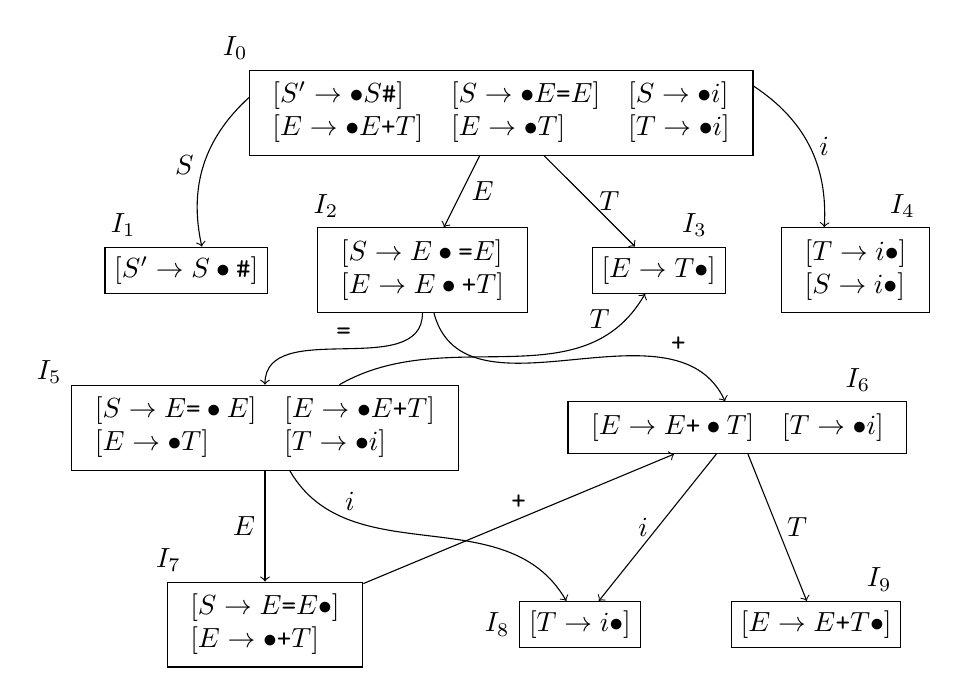
\begin{tikzpicture}
  \node[draw,rectangle,label={170:$I_0$}] (I0) at (0,0) {$\begin{array}{lll}
    [S'\rightarrow\bullet S\texttt{\#}] & [S\rightarrow\bullet E\texttt{=}E] & [S\rightarrow\bullet i]\\\relax
    [E\rightarrow\bullet E\texttt{+}T] & [E\rightarrow\bullet T] & [T\rightarrow\bullet i]
  \end{array}$};
  \node[draw,rectangle,label={150:$I_1$}] (I1) at (-4,-2) {$[S'\rightarrow S\bullet\texttt{\#}]$}; 
  \node[draw,rectangle,label={150:$I_2$}] (I2) at (-1,-2) {$\begin{array}{l}
    [S\rightarrow E\bullet\texttt{=}E]\\\relax
    [E\rightarrow E\bullet\texttt{+}T]\end{array}$};
  \node[draw,rectangle,label={60:$I_3$}] (I3) at (2,-2) {$[E\rightarrow T\bullet]$};
  \node[draw,rectangle,label={60:$I_4$}] (I4) at (4.5,-2) {$\begin{array}{l}
    [T\rightarrow i\bullet]\\\relax
    [S\rightarrow i\bullet]\end{array}$};
  \node[draw,rectangle,label={170:$I_5$}] (I5) at (-3,-4) {$\begin{array}{ll}
    [S\rightarrow E\texttt{=}\bullet E] & [E\rightarrow\bullet E\texttt{+}T]\\\relax
    [E\rightarrow\bullet T] & [T\rightarrow\bullet i]\end{array}$};
  \node[draw,rectangle,label={15:$I_6$}] (I6) at (3,-4) {$\begin{array}{ll}
    [E\rightarrow E\texttt{+}\bullet T] & [T\rightarrow\bullet i]
  \end{array}$};
  \node[draw,rectangle,label={150:$I_7$}] (I7) at (-3,-6.5) {$\begin{array}{l}
    [S\rightarrow E\texttt{=}E\bullet]\\\relax
    [E\rightarrow\bullet\texttt{+}T]
  \end{array}$};
  \node[draw,rectangle,label={180:$I_8$}] (I8) at (1,-6.5) {$[T\rightarrow i\bullet]$};
  \node[draw,rectangle,label={30:$I_9$}] (I9) at (4,-6.5) {$[E\rightarrow E\texttt{+}T\bullet$]};

  \path[->] (I0) [bend right] edge [left] node {$S$} (I1);
  \path[->] (I0) edge [right] node {$E$} (I2) (I0) edge [right] node {$T$} (I3);
  \path[->] (I0) [bend left] edge [right] node {$i$} (I4);
  \path[->] (I2) [out=270,in=90] edge [above] node {$\texttt{=}$} (I5); 
  \path[->] (I5) [out=30,in=240] edge [above,pos=0.8] node {$T$} (I3);
  \path[->] (I2) [out=285,in=115] edge [above,pos=0.8] node {$\texttt{+}$} (I6);
  \path[->] (I5) edge [left] node {$E$} (I7);
  \path[->] (I5) [out=300,in=120] edge [above,pos=0.25] node {$i$} (I8);
  \path[->] (I7) edge [above] node {\texttt{+}} (I6);
  \path[->] (I6) edge [left] node {$i$} (I8);
  \path[->] (I6) edge [right] node {$T$} (I9);
\end{tikzpicture}
\end{document}